%%%%%%%%%%%%%%%%%%%%%%%%%%%%%%%%%%%%%%%%%
% Thin Sectioned Essay
% LaTeX Template
% Version 1.0 (3/8/13)
%
% This template has been downloaded from:
% http://www.LaTeXTemplates.com
%
% Original Author:
% Nicolas Diaz (nsdiaz@uc.cl) with extensive modifications by:
% Vel (vel@latextemplates.com)
%
% License:
% CC BY-NC-SA 3.0 (http://creativecommons.org/licenses/by-nc-sa/3.0/)
%
%%%%%%%%%%%%%%%%%%%%%%%%%%%%%%%%%%%%%%%%%

%----------------------------------------------------------------------------------------
%   PACKAGES AND OTHER DOCUMENT CONFIGURATIONS
%----------------------------------------------------------------------------------------

\documentclass[11pt]{article} % Font size (can be 10pt, 11pt or 12pt) and paper size (remove a4paper for US letter paper)

\usepackage[utf8]{inputenc} % Set utf8 code
\usepackage[protrusion=true,expansion=true]{microtype} % Better typography
\usepackage[portuguese]{babel}
\usepackage{graphicx} % Required for including pictures
\usepackage{wrapfig} % Allows in-line images
\usepackage[pagebackref]{hyperref}

\usepackage{mathpazo} % Use the Palatino font
\usepackage[T1]{fontenc} % Required for accented characters

\usepackage{wallpaper}
\usepackage[font={color=white,bf},figurename=Fig.,labelfont={it}]{caption}
\usepackage{lipsum, xcolor, etoolbox, footmisc, bigfoot}

\usepackage{tabu}
\hypersetup{
    colorlinks=false,
    pdfborder={0 0 0},
}

\setcounter{secnumdepth}{5}
\setcounter{tocdepth}{5}

\linespread{1.05} % Change line spacing here, Palatino benefits from a slight increase by default

\makeatletter
\renewcommand\@biblabel[1]{\textbf{#1.}} % Change the square brackets for each bibliography item from '[1]' to '1.'
\renewcommand{\@listI}{\itemsep=0pt} % Reduce the space between items in the itemize and enumerate environments and the bibliography

\renewcommand{\maketitle}{ % Customize the title - do not edit title and author name here, see the TITLE block below


\begin{center} % Right align
{\LARGE\@title} % Increase the font size of the title

\vspace{20pt} % Some vertical space between the title and author name

\end{center}
}

\patchcmd{\ps@plain}{\thepage}{\textcolor{white}{\thepage}}{}{}
\makeatother

\begin{document}

\ThisTileWallPaper{\paperwidth}{\paperheight}{res/wallpaper_header.jpg}
\color{white}
\pagestyle{plain}
\def\footnotelayout{\color{white}}
\renewcommand\thefootnote{\textcolor{white}{\arabic{footnote}}}
\begin{titlepage}
 \vfill
  \begin{center}
   {\large \textbf{Tiamat}} \\
   {\large \textbf{Babel}}\\
   {\large \href{mailto:tiamatbabel@gmail.com}{tiamatbabel@gmail.com}}\\[6cm]


   {\Large \textbf{GDD}}\\
   {\Large Versão 0.6}\\[6cm]

   \hspace{.45\textwidth} %posiciona a minipage
  \vfill

\vspace{2cm}

\large \textbf{Brasília}

\large \textbf{Abril de 2015}
\end{center}
\end{titlepage}
\newpage

\tableofcontents

\newpage

%----------------------------------------------------------------------------------------
%   DOC BODY
%----------------------------------------------------------------------------------------

\TileWallPaper{\paperwidth}{\paperheight}{res/wallpaper_body.jpg}
\color{white}

\section*{Tabela de Revisão}


\begin{table}[h]

  \taburulecolor{white}
  \color{white}
\begin{tabu}{|l|l|p{60mm}|l|}

\hline 
\textbf{Versão}     & \textbf{Data}     & \textbf{Descrição}                                    & \textbf{Autor}    \\ \hline
0.1                 & 14/04/2015        & Versão inicial                                        & Álex Mesquita     \\ \hline
0.2                 & 15/04/2015        & Requisitos Tecnológicos                               & Álex Mesquita     \\ \hline
0.3                 & 15/04/2015        & Revisão ortográfica                                   & Álex Mesquita     \\ \hline
0.4                 & 25/04/2015        & Front End                                             & Álex Mesquita     \\ \hline
0.5                 & 29/04/2015        & Atualização da imagem de fundo                        & Álex Mesquita     \\ \hline
0.5.1               & 21/05/2015        & Criação das mecânicas do jogo - Exploração vertical   & Jefferson Xavier  \\ \hline
0.5.2               & 21/05/2015        & Criação da Mecânica Exploração horizontal             & Jefferson Xavier  \\ \hline
0.6                 & 21/05/2015        & Finalização das Mecânicas                             & Jefferson Xavier  \\ \hline
0.7                 & 20/06/2015        & Atualização dos Objetivos e criação do Gameplay       & Álex Mesquita     \\ \hline
0.7                 & 10/07/2015        & Criação das estruturas                                & Álex Mesquita     \\ \hline
\end{tabu}
\end{table}

\newpage

\section{Objetivo do jogo}

Babel é um jogo de RPG com temática \textit{Sci-fi}, onde a raça humana vagueia pelo universo na esperança de reconstrução da espécie humana nem novo lar. Após receber um sinal, a raça humana desloca sua nave espacial para um planeta desconhecido à procura desse sinal e acaba encontrando uma torre que definitivamente não podia ter sido construída por humanos. O desafio do jogador será explorar essa torre afim de descobrir seus mistérios, no entanto o jogador deverá explorar o planeta para encontrar e administrar recursos que poderão evoluir as habilidades dos personagens ou serem utilizados para construir equipamentos para facilitar a exploração da torre.

\section{Genêro}

Babel faz uma releitura dos primeiros RPGs clássicos, como Wizardry, trabalhando a questão da exploração em primeira pessoa e sistema de combate clássico de RPGs, porém atualizada com as mecânicas populares de jogos de estratégia e administração de recursos que é amplamente utilizada por jogos atuais voltados a um público mais amplo e diversificado.
 
\section{Visão geral}

O jogo se inicia na base de exploração construída próxima à torre a ser explorada. Nesta base haverá algumas construções essenciais para que o jogador possa evoluir os seus personagens, possibilitando assim montar uma estratégia de exploração da torre e dos recursos contidos no planeta.

A partir da visão de sua base o jogador poderá transitar pelos cenários da torre e da superfície do planeta. Para acessar a torre o jogador deverá clicar sobre um botão de missões na torre que estará disponível no cenário da base. Para retornar à sua base, o jogador deverá concluir ou abortar a missão. Do mesmo modo, para acessar a superfície do planeta, o jogador deverá clicar sobre um botão de missões sobre a superfície da torre que também estará disponível no cenário da base. Ao abrir o cenário da superfície, o jogador poderá selecionar qual missão este irá executar, neste cenário terá um botão para se retornar à base.

O objetivo do jogo é descobrir o propósito da torre e quem construiu esse edifício misterioso. Ao entrar em contato com tal ser, o que ocorreria em seguida? Uma Guerra? Trocas de experiências? Para isso o jogador deverá explorar todos os níveis da torre com os seus personagens. E para facilitar a exploração, será possível coletar \textit{Data points}\footnote{Pontos que serão obtidos através da execução de missões}, podendo assim evoluir os personagens, facilitando o seu desempenho durante as missões na torre. 


\subsection{Gameplay}

\subsubsection{Progressão do Jogo}
A progressão do jogo é não linear, permitindo que o jogador avance no jogo de diversas formas. O jogador começa o jogo em sua colônia, unidade do jogo que apresenta maior neutralidade em relação as dinamicas do jogo, permitindo assim que ele comece a progressão por onde achar mais interessante, exploração horizontal ou vertical. Apesar disso ambas as explorações são intrínsecamente ligadas através do sistema de recursos e progressão de itens e personagens, que criam a interdepêndencia das duas mecânicas numa única dinâmica consisa e original. 

\subsubsection{Objetivo e Estrutura}
O objetivo do jogo é a sobrevivência e restruturação da humanidade num planeta alienígena através da exploração dos seus recursos naturais (planeta/exploração horizontal) e tecnológicos (torre/exploração vertical).

\subsubsection{Exploração Vertical}
A Exploração Vertical consiste na exploração da Torre. Que se vai dar em um formato clássico de Dungeon Crawl, a vista em primeira pessoa e a imersão dada contribui para a experiência de exploração e incerteza, ja que a Torre terá corredores labirintíticos.

\paragraph{Processo da Exploração Vertical} \mbox{}\\
Quando o jogador mostra interesse em explorar a Torre, ele deve antes escolher uma equipe que consiste em 4 Heróis e 1 Drone. Depois de selecionado a equipe e o andar que se deseja explorar, as mecânicas da Exploração Vertical começam a agir.

\paragraph{Exploração e encontros na Exploração Vertical} \mbox{}\\
O andar da Torre é dividida entre quadrados, cada quadrado equivalendo a um comando de movimento do jogador. A disposição dos quadrados irá definir a existência de corredores, salas e outras estruturas dentro da Torre. Todo quadrado poderá ser explorado pelo jogador, caso este consiga vê-lo.

Dentro da Torre há diferentes tipos de encontros. Há o encontro de Combate, encontro de Eventos e a interação entre objetos encontrados dentro da Torre.

\subsubsection{Exploração Horizontal}
A mecânica de exploração horizontal se dará através de menus, numa espécie de hit list, gerando posteriormente a administração dos pontos de interesse do planeta para que o jogador possa gerir os recursos adquiridos.

\subsubsection{Timer}
As diversas ações que o jogador poderá fazer na Base, como Imprimir (construir/comprar) objetos irá demorar uma quantidade de Tempo, tempo imitando a demora para se fazer essa ação. Explorar o planeta também demora uma quantidade de Tempo para ser explorado.

Enquanto as ações demoram uma quantidade X de Tempo para ser realizadas, o jogador é incentivado a passar este tempo na Exploração Vertical, essa mecânica aumenta a dinamicidade entre as mecânicas de Exploração Vertical e Exploração Horizontal.

\subsection{Mecânicas do Jogo}

\subsubsection{Exploração Vertical}
O Jogador explora a Torre por meio de uma equipe composta de 4 heróis e um Drone, a visão do jogo na exploração vertical é em primeira pessoa. Dentro da torre o jogador terá a opção de cumprir quests, interagir com eventos dinâmicos, participar de combates diretos com inimigos e chefes e realizar a progressão da história de acordo com o nível de exploração alcansado.

\begin{figure}[!htp]
\centering
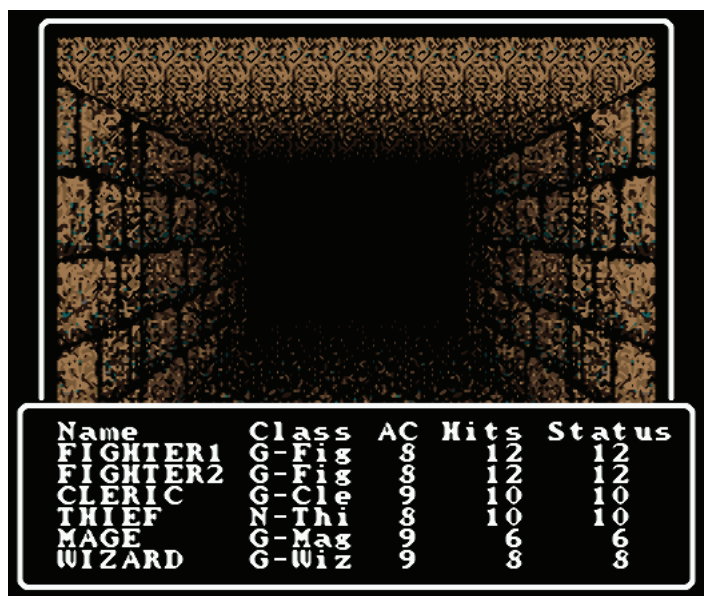
\includegraphics[scale=0.3]{res/Dungeon_Crawler.png}
\caption{Exploração Vertical - Exemplo de Dungeon Crawl}
\label{Exploração Vertical - Exemplo de Dungeon Crawl}
\end{figure}

\paragraph{Movimentação} \mbox{}\\
A movimentação dos personagens na torre se dá através de um grid quadriculado no qual o mapa é projetado, o valor da movimentação é padronizado e contabilizado em unidades, sendo assim um quadrado neste grid corresponde a uma unidade de movimento, essa mecânica é adotada para que a movimentação dentro do labirinto seja mais fluída e precisa.

\subparagraph{Eventos} \mbox{}\\
Os Eventos são acontecimentos dinâmicos situados em pontos específicos da torre, e com resultados diferentes de acordo com a forma como o jogador escolhe interagir com esses eventos. Alguns são permanentes, permitindo que o jogador volte sempre para interagir com aquele objeto/personagem/situação e outros acontecem apenas uma vez.

Os Eventos poderão ser completados de diversas formas, entre eles:

\begin{enumerate}
  \item \textbf{Combate}: Será dada a opção de resolver o conflito por meio de Combate. Utilizando as mecânicas apresentadas de Combate.
  \item \textbf{Valor MPT}: Será dada também a opção de os eventos e conflitos serem resolvidos por meio do Valor MPT do grupo ou de algum indivíduo.
  \item \textbf{Carregar/Ser alguém específico}: Será dada a opção de certos conflitos serem resolvidas por meio de na sua equipe ter algum membro específico de uma classe, ou um item carregado (como uma chave ou relativo a missão).
  \item \textbf{Portas}:
  \begin{itemize}
    \item As portas servirão para dividir espaços dentro da Torre, servindo como divisória entre corredores e salas, por exemplo.
    \item Portas secretas, estas serão invisíveis ao jogador, até que certa ação seja cumprida, seja a derrota de um inimigo específico, a interação entre um objeto dentro da torre como uma alavanca ou a simples necessidade de o jogador estar no quadrado adjacente á porta secreta para esta aparecer.
    \end{itemize}
\end{enumerate}

\paragraph{Encontros} \mbox{}\\
Encontros são divididos entre dois tipos, aleatórios e obrigatórios, os encontros de combate obrigatórios estão citados dentro da lista de eventos e se comportam como tal, já os encontros aleatórios se dão através de uma fórmula fixa padrão, podendo ser alterada em algumas ocasiões para se obter resultados específicos.

A fórmula é 10\% de chance de encontro + 2\% por unidade de movimento, aumentando progressivamente a chance de conflito a cada unidade de movimento percorrida(a cada passo). No entanto esse número é resetado após cada combate, voltando para seu valor inicial de 10\%, caso o jogador fuja do combate ao invés de ir até o fim o valor não é resetado e cai apenas para a metade do valor total do momento do início do combate, logo se o jogador foge de um encontro que se deu aos 40\% de chance, ele volta ao mapa com sua porcentagem reduzida a 20\%.

\newpage

\subsubsection{Exploração Horizontal}
A exploração horizontal se dá através de uma lista de quests a serem completadas nos pontos de interesse já conhecidos e de novos pontos de interesse a ser descobertos. Exigindo que o jogador escolha entre a segurança e estabilidade de gerenciar/administrar pontos de interesse já conhecidos(sistema de quests/eventos) ou que o jogador arrisque a segurança da equipe, recursos e tempo na descoberta de novos pontos de interesse.

\begin{figure}[!htp]
\centering
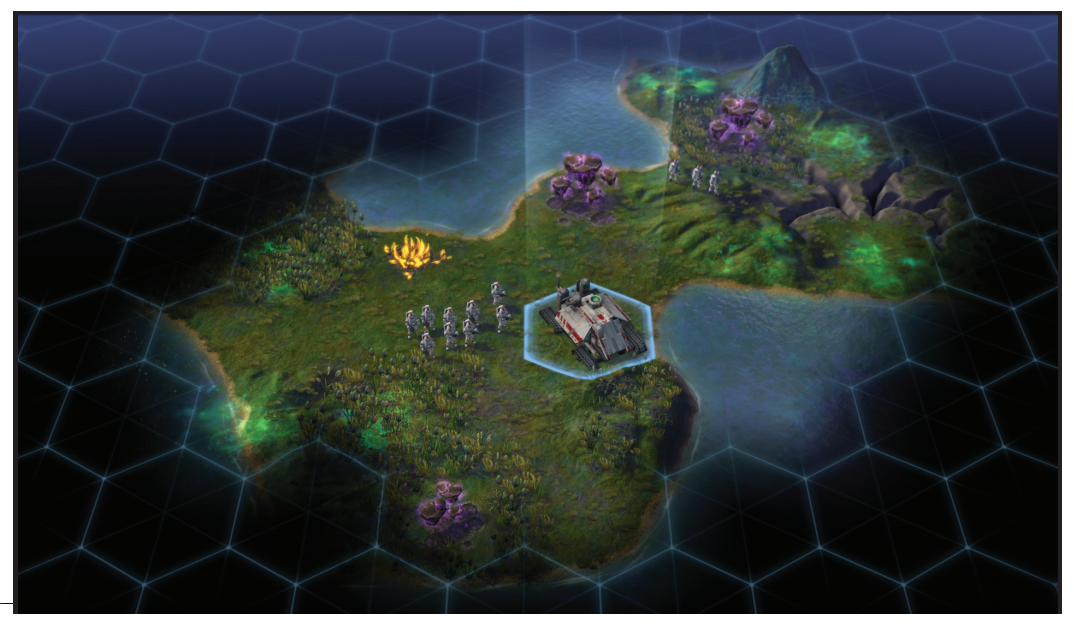
\includegraphics[scale=0.3]{res/resources.png}
\caption{Exemplo de Exploração Horizontal}
\label{Exemplo de Exploração Horizontal}
\end{figure}

\paragraph{Espaço} \mbox{}\\
A Exploração Horizontal se dá na superfície do planeta.
\paragraph{Locais} \mbox{}\\
Os pontos de interesse são pré estabelecidos, tendo alguns fixos(para fins de balanceamento de progressão do jogador).

Estes locais estarão posicionados em uma malha virtual abstrata, posicionadas nos vértices desta mesma malha. A cada local explorado, é revelado no mapa do planeta todos os locais que ligam aquele local na malha, aumentando as possibilidades e locais de exploração.

No total serão 15 pontos de interesse, cada um com no mínimo um evento e entre 1 e 5 quests, o número de quests por ponto de interesse será definido de acordo com a nossa capacidade de implementação de conteúdo e com a possível relevância daquele ponto de interesse.

\paragraph{Resolução} \mbox{}\\
Cada ponto de interesse contará com desafios próprios para que seja considerado um lugar explorado, majoritariamente a resolução desses conflitos vai se dar de forma simples de comparação de valores, cada local inexplorado vai contar com valores X de M, P e T fixos e invisíveis para o jogador. Esses valores deverão ser igualados ou superados pela equipe exploradora para que a missão seja considerada um sucesso e o ponto de interesse seja revelado. Existem nuances no entanto em relação a essa resolução e 3 condições distintas de vitória e derrota, baseadas em quantos valores a equipe de exploração tem iguais ou mais elevados que os valores propostos pelo desafio.

Condições de vitória e derrota:
\begin{itemize}
  \item \textbf{3 valores iguais ou superiores} - Nem os personagens nem os veículos sofrem danos, metade dos recursos de matéria e energia investidos na missão são retornados ao jogador, a zona desconhecida se torna um ponto de interesse.
  \item \textbf{2 valores iguais ou superiores} - Os personagens/veículo sofrem dano de 10\% de hp e todos os recursos utilizados na exploração são gastos, a zona desconhecida se torna um ponto de interesse.
  \item \textbf{1 valor igual ou superior} - Metade dos personagens envolvidos na exploração morrem, o veículo é reduzido a 50\% de sua durabilidade(a questão de durabilidade ainda vai ser discutida no entanto, devido a quantidade de conteúdos com prioridade na lista de implementação) todos os recursos são gastos, a zona desconhecida permanecerá desconhecida.
  \item \textbf{0 valores iguais ou superiores} - Todos seus personagens morrem, o veículo é perdido, todos os recursos são gastos e a zona permanece desconhecida.
\end{itemize}

\subsection{Colônia}

\begin{figure}[!htp]
\centering
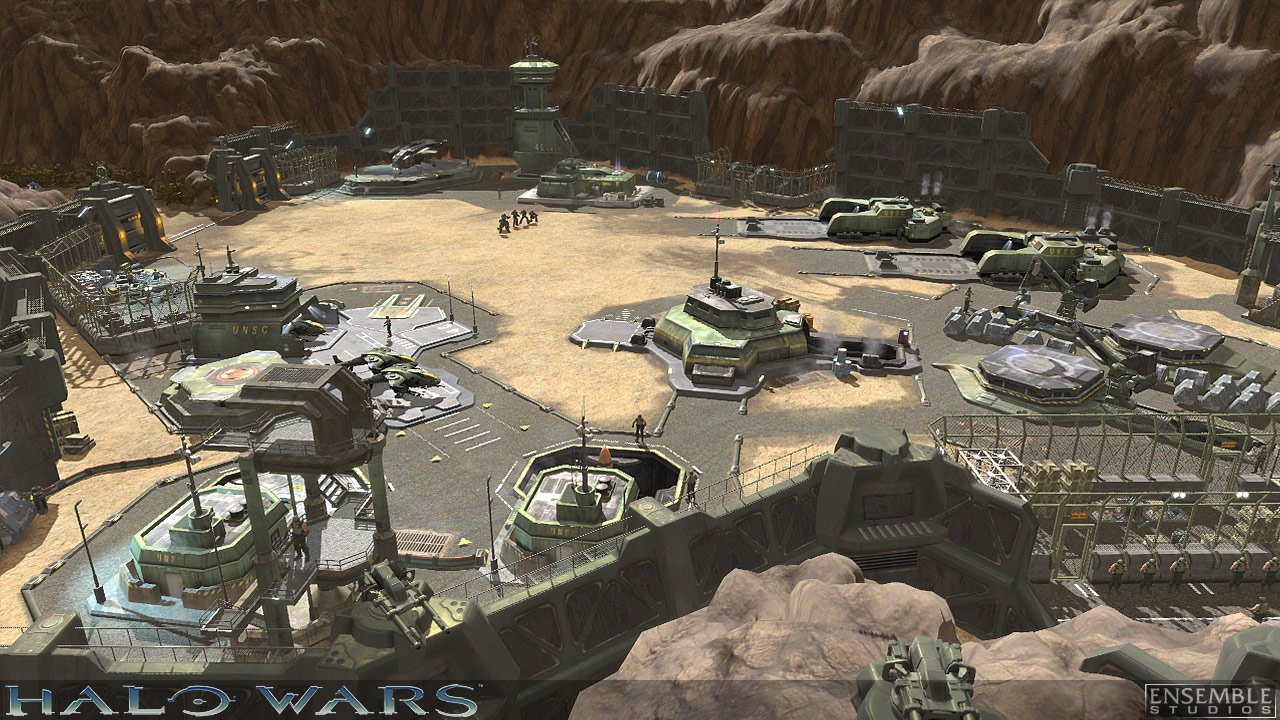
\includegraphics[scale=0.3]{res/base_building.png}
\caption{Exemplo de Colônia}
\label{Exemplo de Base Building}
\end{figure}

\subsubsection{Recursos}

O jogo contará com 3 recursos distintos para realizar a progressão da base e dos personagens, sendo eles Data, Matéria e Energia.

\subsubsection{Estrutura}

\paragraph{Barracks} \mbox{}\\
Estrutura fundamental para desenvolvimento dos personagens, todo o planejamento em relação a habilidades, equipamento e equipe são feitos nesta tela.

Funções:
\begin{itemize}
  \item \textbf{Chat} - Hank,  supervisor geral do centro de treinamento de forças especiais, um homem certamente muito habilidoso e respeitado.
  \item \textbf{Inspect} - Tela para analisar o status do seu personagem e avançar de nível.
  \item \textbf{Equip} - Tela para equipar e comprar equipamentos.
  \item \textbf{Party} - Tela para se escolher a equipe que vai fazer a exploração da torre.
\end{itemize}


\paragraph{Facilities} \mbox{}\\
Estrutura de upgrades gerais, habilita schematics e habilidades passivas.

Funções:
\begin{itemize}
  \item \textbf{Chat}
    \begin{enumerate}
      \item \textbf{Militar} - Bowie, homem loiro e de grande porte/estatura porém levemente gentil.
      \item \textbf{Psiônico} - Ripley, mulher magra, misteriosa, com aparencia frágil e com roupas coladas cabelos ruivos. 
      \item \textbf{Tecnológico} - Connor, Hacker numa colônia espacial
    \end{enumerate}
  \item \textbf{Militar} - Tela onde os personagens militares que estão em criogenia serão acordados, para cada 15 personagens acordados o level das armas do tipo militar terão um acrescimo de uma unidade.
  \item \textbf{Psiônico} - Tela onde os personagens psiônicos que estão em criogenia serão acordados, para cada 15 personagens acordados o level das armas do tipo psiônico terão um acrescimo de uma unidade.
  \item \textbf{Tecnológico} - Tela onde os personagens tecnológicos que estão em criogenia serão acordados, para cada 15 personagens acordados o level das armas do tipo tecnológico terão um acrescimo de uma unidade.
\end{itemize}

\paragraph{Hospital} \mbox{}\\
Estrutura onde se compra itens, cura e revive os personagens e se realiza novas pesquisas tanto de medicamentos e genética. 

Funções:
\begin{itemize}
  \item \textbf{Chat} - Doutora Anne C. Clarke, Loira olhos azuis, óculos, cabelo preso com rabo de cavalo, jaleco.
  \item \textbf{Itens} - Medicamentos de cura, aumento de potencial humano. 
  \item \textbf{Research} - Pesquisa dos itens através de pesquisas liberadas em facilities e descobertas da torre.
  \item \textbf{Revive} - Cura personagens e revive os mortos. 
\end{itemize}

\subsubsection{Pesquisas}
\subsubsection{NPCs}

\subsection{Combate}

\newpage


\section{Esquema de controle e interface com o usuário}

Na exploração vertical, no interior da torre, esta será em primeira pessoa, sendo que serão utilizadas as teclas destacadas na figura a seguir:\\

\begin{figure}[!htp]
\centering
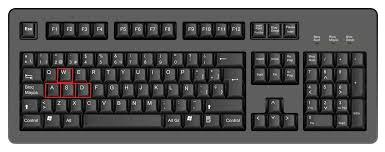
\includegraphics[scale=0.75]{res/keyboard.jpg}
\caption{Teclas utilizadas}
\label{Teclado}
\end{figure}

Onde a tecla ''w'' irá movimentar o jogador para frente, a tecla ''s'' irá movimentar o jogador para trás, a tecla ''a'' irá rotacionar o jogador $90\,^{\circ}$ para a esquerda e a tecla ''d'' irá rotacionar o jogador $90\,^{\circ}$ para a direita. A tecla ''e'' será utilizada para interação dos objetos com o personagem.

Na exploração horizontal, a superfície do planeta, o jogador irá usar o \textit{mouse} para navegar na superfície, utilizando o botão esquerdo para selecionar objetos e executar todas as ações na base e superfície do planeta. Na exploração vertical, no interior da torre, o botão esquerdo servirá para realizar a ação principal do personagem.

\begin{figure}[!htp]
\centering
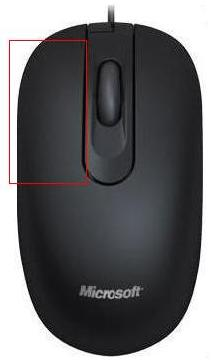
\includegraphics[scale=0.4]{res/mouse.jpg}
\caption{Mouse}
\label{Mouse}
\end{figure}

\section{Front End}

O \textit{Front End} representa as tela que serão carregadas assim que o jogo é iniciado. A seguir serão ilustradas cada uma das telas que serão apresentadas ao iniciar o \textbf{Babel}.

A logo a seguir representa a empresa responsável por desenvolver o jogo.

\begin{figure}[!htp]
\centering

\includegraphics[scale=0.6]{res/tiamat_logo.png}
\caption{Logo da Tiamat}
\label{Logo da Tiamat}
\end{figure}

A logo a seguinte representa a API utilizada durante o desenvolvimento.

\begin{figure}[!htp]
\centering

\includegraphics[scale=0.6]{res/Sdl-logo.png}
\caption{Logo da SDL}
\label{Logo da SDL}
\end{figure}

A imagem a seguir representa a classificação indicativa para o jogadores.

\newpage

\begin{figure}[!htp]
\centering

\includegraphics[scale=0.5]{res/classification.png}
\caption{Classificação Indicativa}
\label{Classificação Indicativa}
\end{figure}

\section{Requisitos Tecnológicos}

\begin{figure}[tb]
\begin{center}
  
\includegraphics[scale=0.3]{res/cubase-Logo.png} \quad
  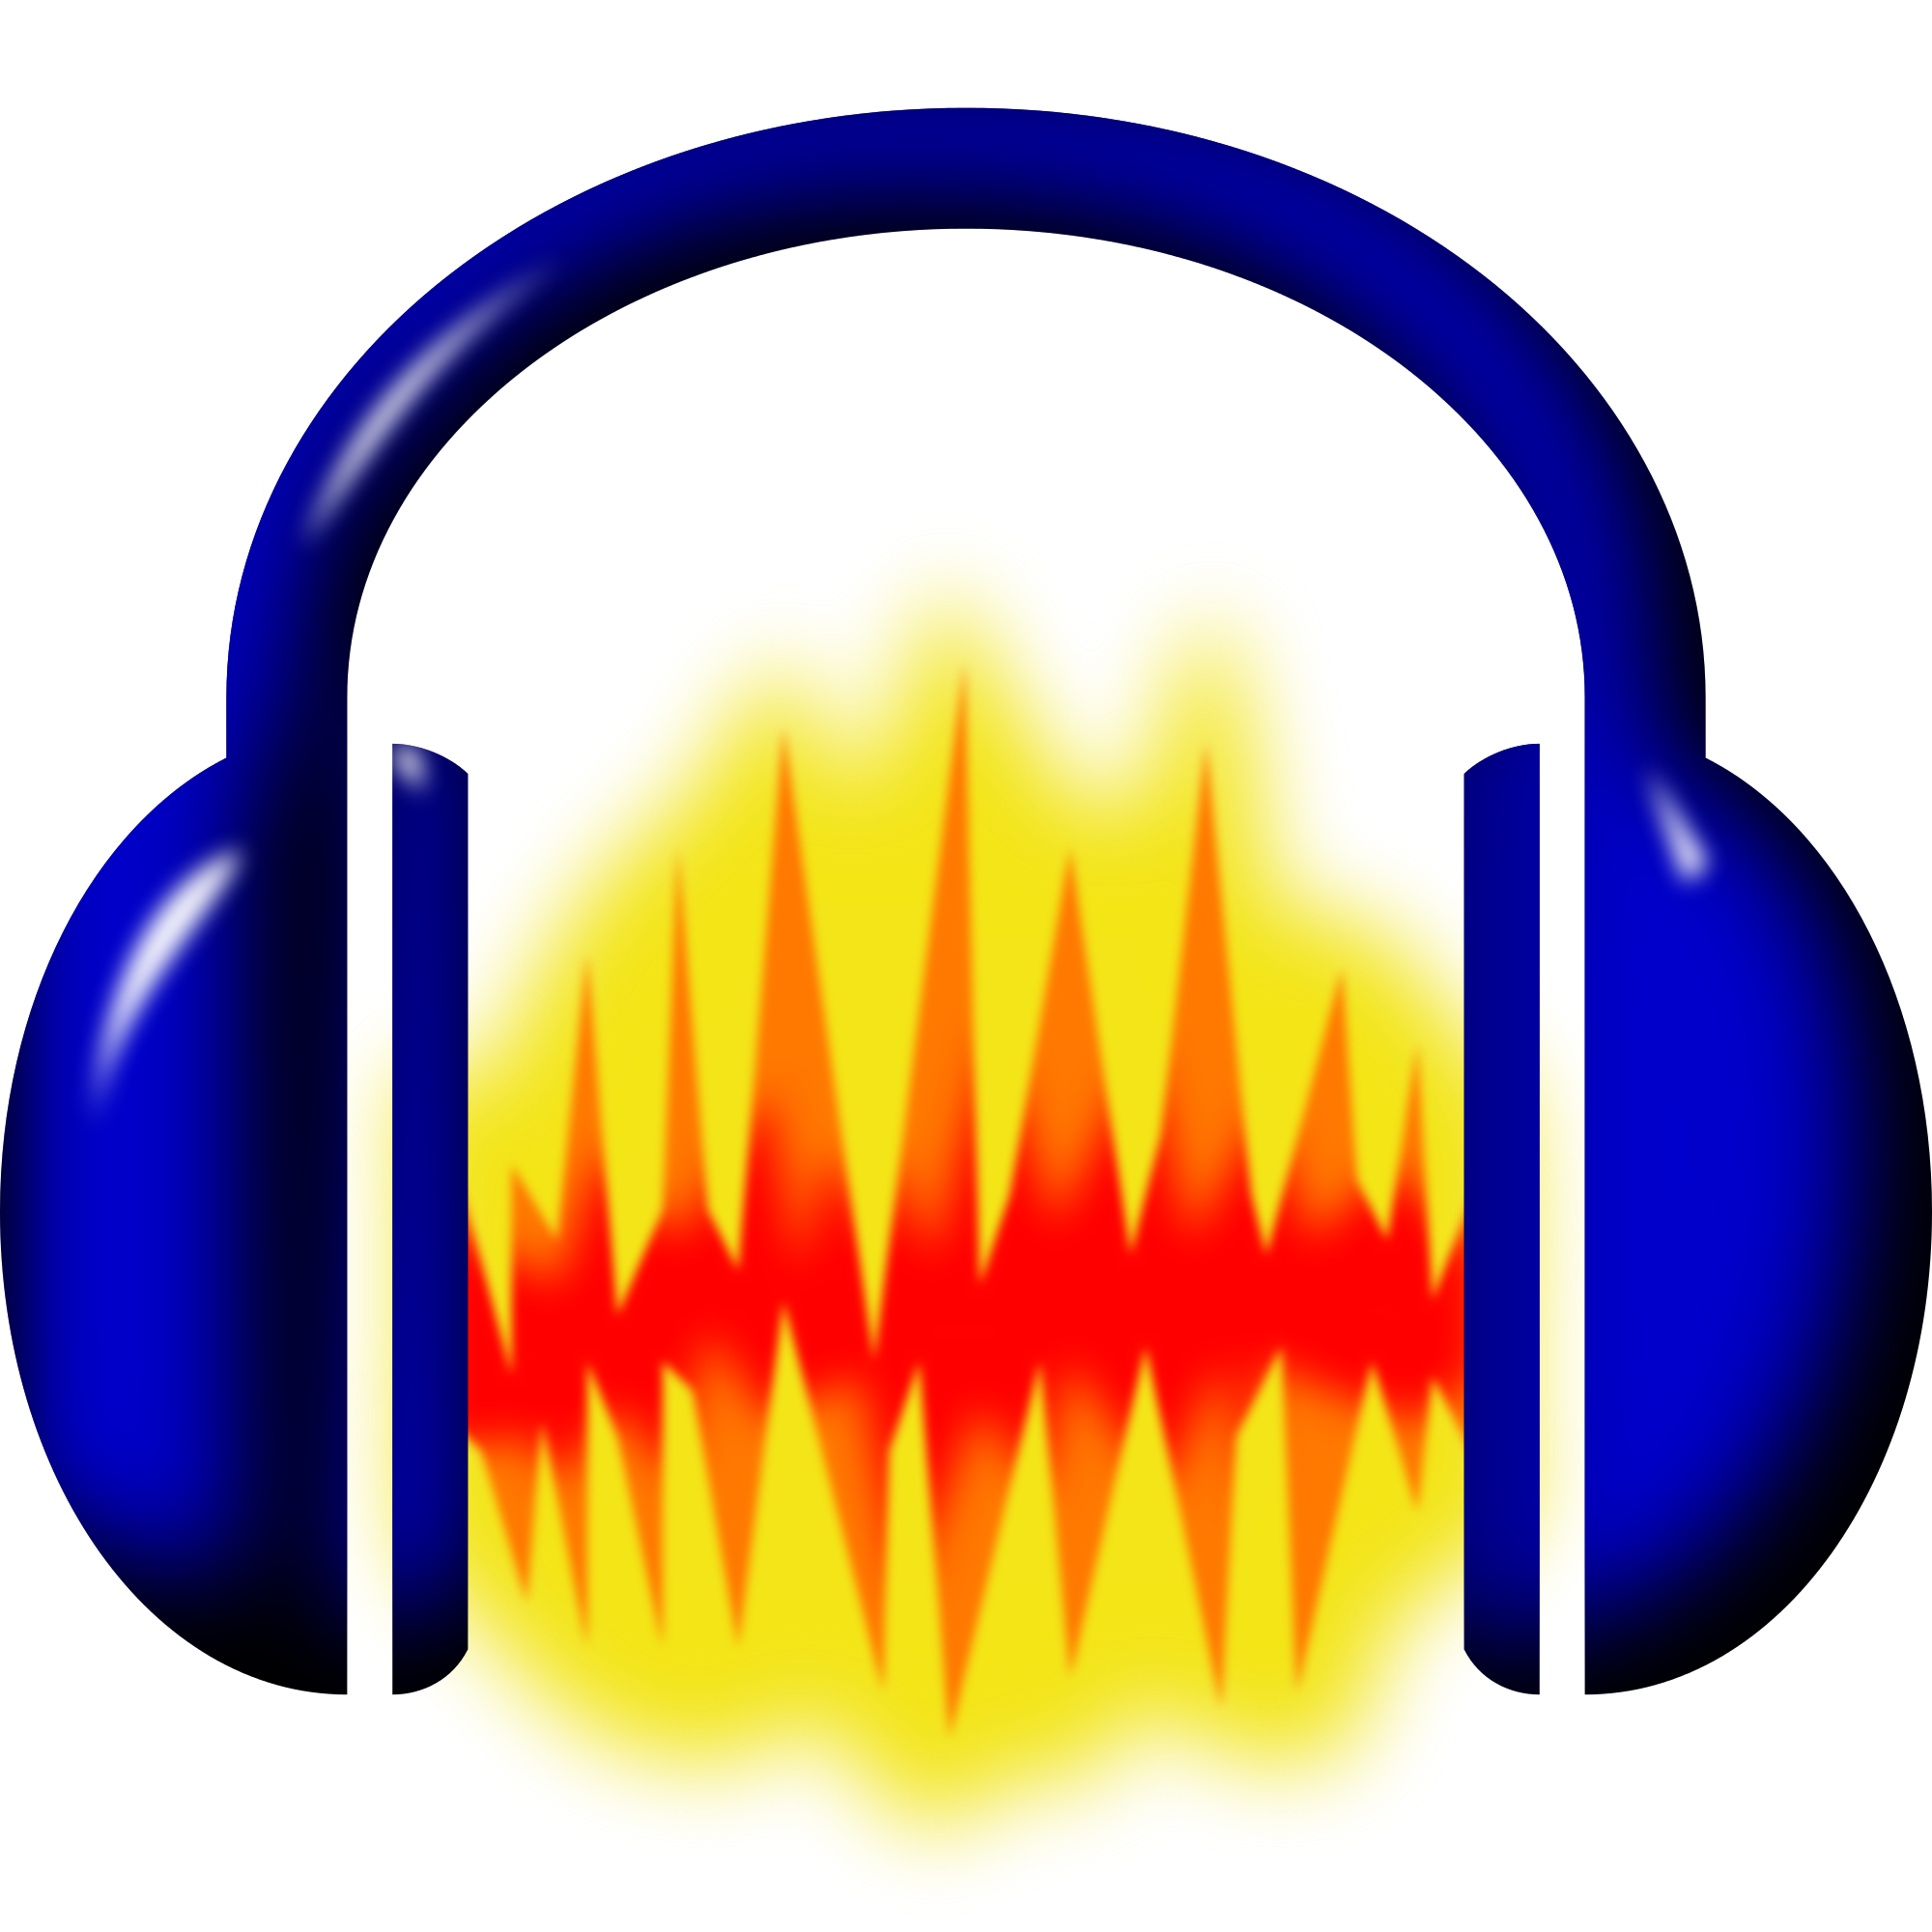
\includegraphics[scale=0.04]{res/audacity.png} \quad
  
\includegraphics[scale=0.3]{res/adobe_illustrator.png} \quad
  
\includegraphics[scale=0.25]{res/Sdl-logo.png} \quad
  
\includegraphics[scale=0.3]{res/Sublime_Text_Logo.png} \quad
  
\includegraphics[scale=0.2]{res/cpp.png} \quad
  
\includegraphics[scale=0.13]{res/git.png} \quad
  
\includegraphics[scale=0.15]{res/lua.png} \quad
  
\includegraphics[scale=0.4]{res/GDB.png} \quad
  
\includegraphics[scale=0.16]{res/linux.png} \quad
  
\includegraphics[scale=0.35]{res/GCC.png} \quad
  
\includegraphics[scale=0.05]{res/windows.png} \quad
\caption{Requisitos Tecnológicos} \label{gdimotes}
\end{center}
\end{figure}

\end{document}
